\documentclass{beamer}
\usetheme{Boadilla}

\makeatother
\setbeamertemplate{footline}
{
    \leavevmode%
    \hbox{%
    \begin{beamercolorbox}[wd=.4\paperwidth,ht=2.25ex,dp=1ex,center]{author in head/foot}%
        \usebeamerfont{author in head/foot}\insertshortauthor
    \end{beamercolorbox}%
    \begin{beamercolorbox}[wd=.55\paperwidth,ht=2.25ex,dp=1ex,center]{title in head/foot}%
        \usebeamerfont{title in head/foot}\insertshorttitle
    \end{beamercolorbox}%
    \begin{beamercolorbox}[wd=.05\paperwidth,ht=2.25ex,dp=1ex,center]{date in head/foot}%
        \insertframenumber{}
    \end{beamercolorbox}}%
    \vskip0pt%
}
\makeatletter
\setbeamertemplate{navigation symbols}{}

\usepackage[T1]{fontenc}
\usepackage{lmodern}
\usepackage{amssymb,amsmath}
\renewcommand{\familydefault}{\sfdefault}

\DeclareMathOperator*{\argmax}{argmax}

\usepackage{mathtools}
\usepackage{graphicx}
\usepackage{threeparttable}
\usepackage{booktabs}
\usepackage{siunitx}
\sisetup{parse-numbers=false}

%\setlength{\OuterFrameSep}{-2pt}
%\makeatletter
%\preto{\@verbatim}{\topsep=-10pt \partopsep=-10pt }
%\makeatother

\title[Lecture 22:\ Dynamic Discrete Choice II]{Lecture 22:\ Dynamic Discrete Choice II}
\author[ResEcon 703:\ Advanced Econometrics]{ResEcon 703:\ Topics in Advanced Econometrics}
\date{Matt Woerman\\University of Massachusetts Amherst}

\begin{document}

{\setbeamertemplate{footline}{} 
\begin{frame}[noframenumbering]
    \titlepage
\end{frame}
}

\begin{frame}\frametitle{Agenda}
    Last time
    \begin{itemize}
        \item Dynamic Discrete Choice
    \end{itemize}
    \vspace{2ex}
    Today
    \begin{itemize}
        \item Rust (1987)
    \end{itemize}
    \vspace{2ex}
    Upcoming
    \begin{itemize}
        \item Reading for next time
        \begin{itemize}
            \item Train textbook, Chapter 13
            \item Nevo and Whinston (2010)
        \end{itemize}
        \item Problem sets
        \begin{itemize}
            \item Problem Set 4 is due
        \end{itemize}
        \item Final exam
        \begin{itemize}
        	\item More information next time
        \end{itemize}
    \end{itemize}
\end{frame}

\begin{frame}\frametitle{Dynamic Discrete Choice}
    Many optimization problems have a dynamic component
    \begin{itemize}
    	\item A choice made today affects the choice set or utility of choices in the future
    	\item When making a choice today, a decision maker considers not only the current utility of each alternative but also future effects
    \end{itemize}
    \vspace{2ex}
    Example: College
    \begin{itemize}
    	\item Attending college may generate less utility than working, joining the Peace Corps, hiking the Trans-Canada Trail, or whatever else an 18-year-old might want to do
    	\item But attending college opens up future career opportunities and salaries that may not exist after these other alternatives
    \end{itemize}
    \vspace{2ex}
    Dynamic models have an additional layer of complexity that often require more advanced estimation methods
\end{frame}

\begin{frame}\frametitle{}
    \vfill
    \centering
    \begin{beamercolorbox}[center]{title}
        \Large Rust (1987)
    \end{beamercolorbox}
    \vfill
\end{frame}

\begin{frame}\frametitle{An Empirical Model of Harold Zurcher}
    This paper develops a dynamic discrete choice model to describe the behavior of Harold Zurcher
    \begin{itemize}
    	\item Superintendent of maintenance at the Madison (Wisconsin) Metropolitan Bus Company
    	\item Responsible for determining when to replace municipal bus engines
    \end{itemize}
    \vspace{2ex}
    Why do we care about Harold Zurcher and bus engine replacement?
    \begin{itemize}
    	\item We don't, \emph{per se}, but this application provides a framework to illustrate two ideas
    	\begin{itemize}
    		\item Bottom-up (or microfounded) model of a dynamic investment/replacement decision
    		\item Nested fixed point algorithm for estimating dynamic discrete choice models
   		\end{itemize}
    \end{itemize}
\end{frame}

\begin{frame}\frametitle{Bus Engine Replacement Decision}
    Each month and for each city bus, Harold Zurcher must choose between two alternatives
    \begin{itemize}
    	\item Perform routine maintenance on the bus engine
    	\item Replace the bus engine
    \end{itemize}
    \vspace{2ex}
    Harold Zurcher faces a tradeoff between these two choices
    \begin{itemize}
    	\item Routine engine maintenance is relatively inexpensive
    	\item Engine replacement is more expensive but reduces the probability of a costly breakdown
    \end{itemize}
    \vspace{2ex}
    Harold considers a bus engine's mileage and other factors to determine when it is time to replace the engine
\end{frame}

\begin{frame}\frametitle{Data}
    Data on bus mileage and maintenance
    \begin{itemize}
    	\item 162 buses in the Madison Metro fleet
    	\item Data for the period December, 1974 to May, 1985
    	\item Monthly observations of mileage (odometer readings) for each bus
    	\item Maintenance log with date, mileage, and repair description
    \end{itemize}
\end{frame}

\begin{frame}\frametitle{Model: Variable Definitions}
    State variable: $x_t$, a bus engine's mileage in month $t$
    \begin{itemize}
    	\item A state variable describes the state of the dynamic system
    	\item Mileage is a continuous variable that Rust discretizes into 90 bins for tractability
    \end{itemize}
    \vspace{2ex}
    Choice variable: $i_t \in \{0, 1\}$ defines bus engine replacement
    \begin{align*}
    	i_t = 0 \quad &\Rightarrow \quad \text{perform routine engine maintenance in month } t \\
    	i_t = 1 \quad &\Rightarrow \quad \text{replace the bus engine in month } t
    \end{align*} \\
    \vspace{2ex}
    Transition probability: $p(x_{t+1} \mid x_t, i_t, \theta_3)$ governs the evolution of $\{x_t\}$
    $$p(x_{t+1} \mid x_t, i_t, \theta_3) = 
    	\begin{cases}
    		\theta_3 e^{\theta_3 (x_{t+1} - x_t)} & \text{if } i_t = 0\\
    		\theta_3 e^{\theta_3 x_{t+1}} & \text{if } i_t = 1
    	\end{cases}$$ \\	
    \begin{itemize}
    	\item Probability of mileage next month conditional on mileage this month, the maintenance/replacement decision, and a parameter
    \end{itemize}
\end{frame}

\begin{frame}\frametitle{Model: Utility and Cost Functions}
    Harold Zurcher's utility function (or the Madison Metro profit function) for each bus in the fleet is
    $$u(x_t, i_t, \theta_1) = 
    	\begin{cases}
    		-c(x_t, \theta_1) & \text{if } i_t = 0 \\
    		-[RC + c(0, \theta_1)] & \text{if } i_t = 1
    	\end{cases}$$
    where
    \begin{itemize}
    	\item $c(\cdot, \theta_1)$ is the cost of routine engine maintenance (including the expected cost of a breakdown)
    	\item $\theta_1$ is a parameter that defines the cost function
    	\item $RC$ is the engine replacement cost
    \end{itemize}
\end{frame}

\begin{frame}\frametitle{Model: Value Function}
    The value function is defined as the unique solution to the Bellman Equation
    \begin{align*}
    	V_{\theta}(x_t) &= \max_{i_t} [u(x_t, i_t, \theta_1) + \beta EV_{\theta}(x_t, i_t)] \\
    	\intertext{where}
    	EV_{\theta}(x_t, i_t) &= \int V_{\theta}(y) p(dy \mid x_t, i_t, \theta_3)
    \end{align*}
\end{frame}

\begin{frame}\frametitle{Approach 1: Solution}
    There is an optimal replacement policy that solves this Bellman Equation
    $$i_t = f(x_t, \theta) = 
    	\begin{cases}
    		0 & \text{if } x_t \leq \gamma(\theta) \\
    		1 & \text{if } x_t > \gamma(\theta)
    	\end{cases}$$
    where $\gamma(\theta)$ is the unique solution to
    $$(1 - \beta) RC = \int_0^{\gamma(\theta)} \left[ 1 - \beta e^{-\theta_3 (1 - \beta) y} \right] \frac{\partial c(y, \theta_1)}{\partial y} dy$$ \\
    \vspace{2ex}
    $\gamma(\theta)$ is a constant (conditional on $\theta_1$ and $\theta_3$) that defines the threshold for optimal bus engine replacement
    \begin{itemize}
    	\item Whenever mileage exceeds $\gamma(\theta)$, it is optimal to replace the engine
    \end{itemize}
\end{frame}

\begin{frame}\frametitle{Approach 1: Problems}
    The data do not reflect this result that all bus engines are replaced when they cross a constant mileage threshold
    \begin{itemize}
    	\item Mileage at replacement varies from 82,400 miles to 387,300 miles
    \end{itemize}
    \vspace{2ex}
    We can rationalize these data by assuming Harold Zucher has additional knowledge of the state of a bus engine, $\varepsilon_t$, that he uses to determine if a bus engine should be replaced
    $$i_t = f(x_t, \theta) + \varepsilon_t$$ \\
    \vspace{2ex}
    This equation reflects a ``reduced-form'' error term
    \begin{itemize}
    	\item This error term is internally inconsistent with our structural model
    	\item The error term should enter into Harold Zucher's optimization, not simply be tacked on at the end
    \end{itemize}
\end{frame}

\begin{frame}\frametitle{Approach 2: Model}
    The second approach to solving this model adds the error term into the Bellman Equation
    \begin{align*}
    	V_{\theta}(x_t, \varepsilon_t) &= \max_{i_t} [u(x_t, i_t, \theta_1) + \varepsilon_t(i_t) + \beta EV_{\theta}(x_t, \varepsilon_t, i_t)] \\
    	\intertext{where}
    	EV_{\theta}(x_t, \varepsilon_t, i_t) &= \int_y \int_\eta V_{\theta}(y, \eta) p(dy, d \eta \mid x_t, \varepsilon_t, i_t, \theta_2, \theta_3)
    \end{align*} \\
    \begin{itemize}
    	\item $p(x_{t+1}, \varepsilon_{t+1} \mid x_t, \varepsilon_t, i_t, \theta_2, \theta_3)$ is the transition density for $(x_t, \varepsilon_t)$
    	\item $\theta_2$ is a new parameter that governs the joint evolution of $x_t$ and $\varepsilon_t$
    \end{itemize}
    \vspace{2ex}
    $\varepsilon_t$ is an unobserved state variable, which adds complexity to estimation
\end{frame}

\begin{frame}\frametitle{Conditional Independence Assumption}
    The transition density of the controlled process $\{x_t, \varepsilon_t\}$ factors as
    $$p(x_{t+1}, \varepsilon_{t+1} \mid x_t, \varepsilon_t, i_t, \theta_2, \theta_3) = q(\varepsilon_{t+1} \mid x_{t+1}, \theta_2) p(x_{t+1} \mid x_t, i_t, \theta_3)$$ \\
    \vspace{2ex}
    Any correlation between $\varepsilon_t$ and $\varepsilon_{t+1}$ can be captured by $x_{t+1}$
    \begin{itemize}
    	\item The $\{\varepsilon_t\}$ is essentially noise superimposed on the $\{x_t\}$ process
    \end{itemize}
    \vspace{2ex}
    We can further simplify the problem by assuming $\varepsilon_t$ is i.i.d.\ extreme value
    \begin{itemize}
    	\item Any additional information known to Harold Zurcher (but unobserved by us) can be treated as random noise
    \end{itemize}
    \vspace{2ex}
    These assumptions greatly reduce the curse of dimensionality and yield closed-form expressions for choice probabilities
\end{frame}

\begin{frame}\frametitle{Theorems 1 and 2}
    The choice probability of the bus engine replacement decision is
    \begin{align*}
    	P(i_t \mid x_t, \theta) &= \frac{e^{u(x_t, i_t, \theta_1) + \beta EV_{\theta}(x_t, i_t)}}{\sum_{j_t \in \{0, 1\}} e^{u(x_t, j_t, \theta_1) + \beta EV_{\theta}(x_t, j_t)}} \\
    	\intertext{where $EV_{\theta}$ is the unique solution to}
    	EV_{\theta}(x_t, i_t) &= \int \ln \left[ \sum_{j_t \in \{0, 1\}} e^{u(y, j_t, \theta_1) + \beta EV_{\theta}(y, j_t)} \right] p(dy \mid x_t, i_t, \theta_3)
    \end{align*} \\
    \vspace{2ex}
    The likelihood function is given by
    $$\ell^f(x_1, \ldots, x_T, i_1, \ldots, i_T \mid x_0, i_0, \theta) = \prod_{t = 1}^T P(i_t \mid x_t, \theta) p(x_t \mid x_{t-1}, i_{t-1}, \theta_3)$$
\end{frame}

\begin{frame}\frametitle{Estimating the Model}
    This model is estimated by maximum likelihood using a nested fixed point algorithm
    \begin{itemize}
    	\item The likelihood function depends on choice probabilities
    	\item Choice probabilities depend on the value function, which is unknown
    	\item Conditional on a set of parameters, a nested fixed point algorithm solves for the value function
    \end{itemize}
    \vspace{2ex}
    Two loops for estimation
    \begin{itemize}
    	\item Outer loop find the values of $\theta$ that maximize the likelihood function
    	\item Within each iteration of the outer loop, an inner loop uses a nested fixed point algorithm to find the value function $EV_{\theta}$
    \end{itemize}
\end{frame}

\begin{frame}\frametitle{Value Function Fixed Point}
    We need to find the value function for a set of parameters
    $$EV_{\theta}(x_t, i_t) = \int \ln \left[ \sum_{j_t \in \{0, 1\}} e^{u(y, j_t, \theta_1) + \beta EV_{\theta}(y, j_t)} \right] p(dy \mid x_t, i_t, \theta_3)$$ \\
    \begin{itemize}
    	\item Rust discretizes $x_t$ into 90 mileage bins, so we want to find a value of $EV_{\theta}$ for each of those bins
    \end{itemize}
    \vspace{2ex}
    $EV_{\theta}$ is also on the right-hand side of this equation, so we want to find the fixed point
    \begin{itemize}
    	\item We want to find the $EV_{\theta}$ function that, when put into the right-hand side of the equation, is also what is returned on the left-hand side of the equation
    \end{itemize}
\end{frame}

\begin{frame}\frametitle{Nested Fixed Point Algorithm}
    Three steps to estimate this model
    \begin{enumerate}
    	\item Impute a value of the discount factor, $\beta$
    	\item Estimate $\theta_3$, the parameters of the transition probabilities, which can be done without the behavioral model of Harold Zurcher
    	\item Outer loop: search over $(\theta_1, RC)$ to maximize the likelihood function
    	\begin{enumerate}
    		\item Inner loop: find the fixed point of the value function conditional on $(\beta, \theta_1, \theta_3, RC)$
    		\item Use this value function to calculate choice probabilities and then likelihood
    	\end{enumerate}
    \end{enumerate}
\end{frame}

\begin{frame}\frametitle{Structural Estimates}
	\centering
    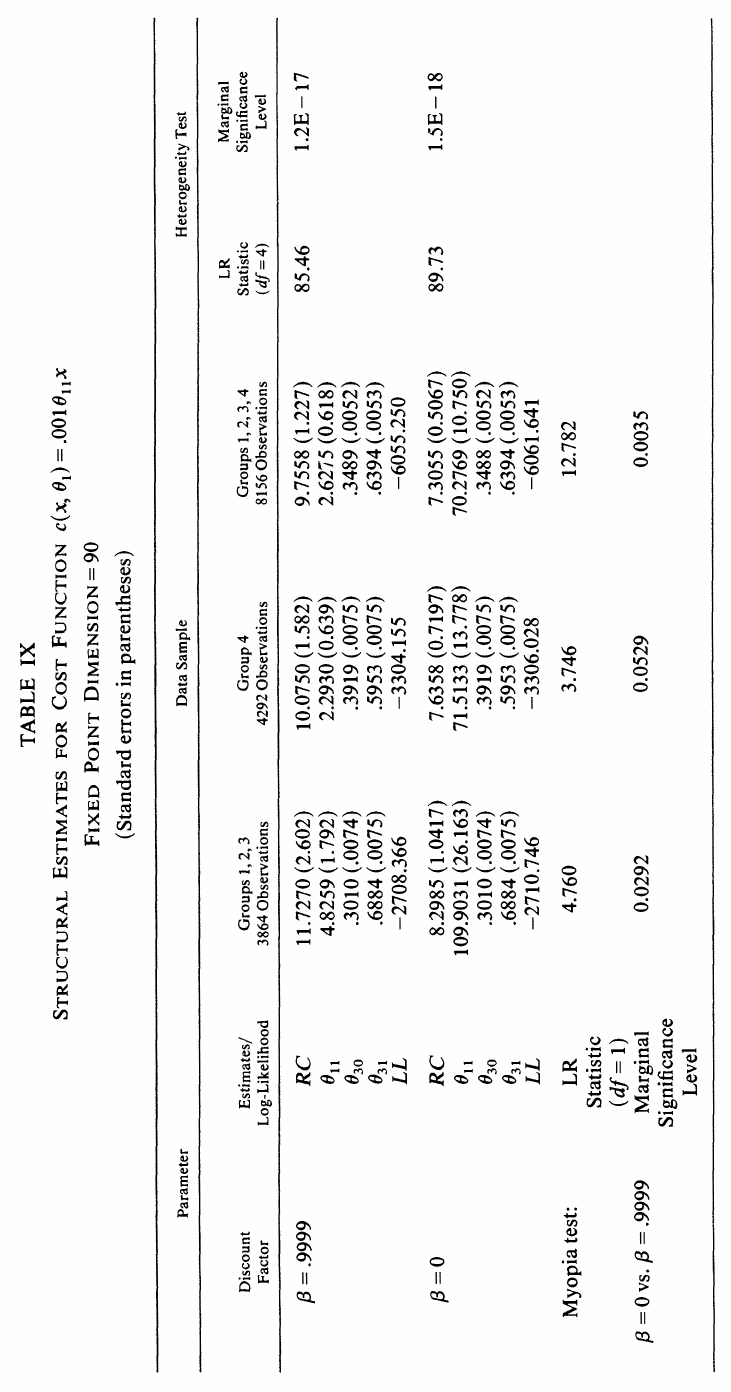
\includegraphics[angle=270, width=\textwidth]{estimates.png}
\end{frame}

\begin{frame}\frametitle{Value Function}
	\centering
    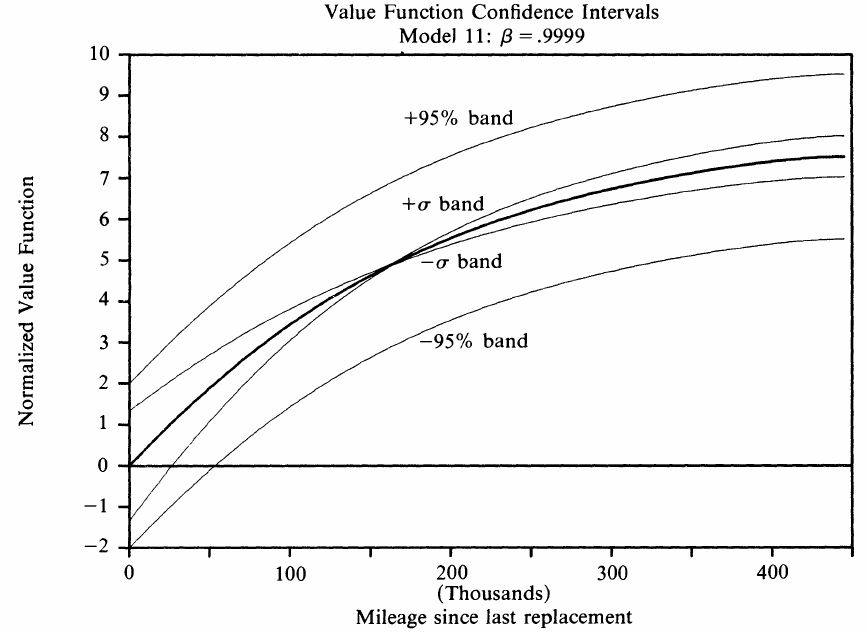
\includegraphics[width=0.9\textwidth]{value_function.png}
\end{frame}

\begin{frame}\frametitle{Probability of Engine Replacement}
	\centering
    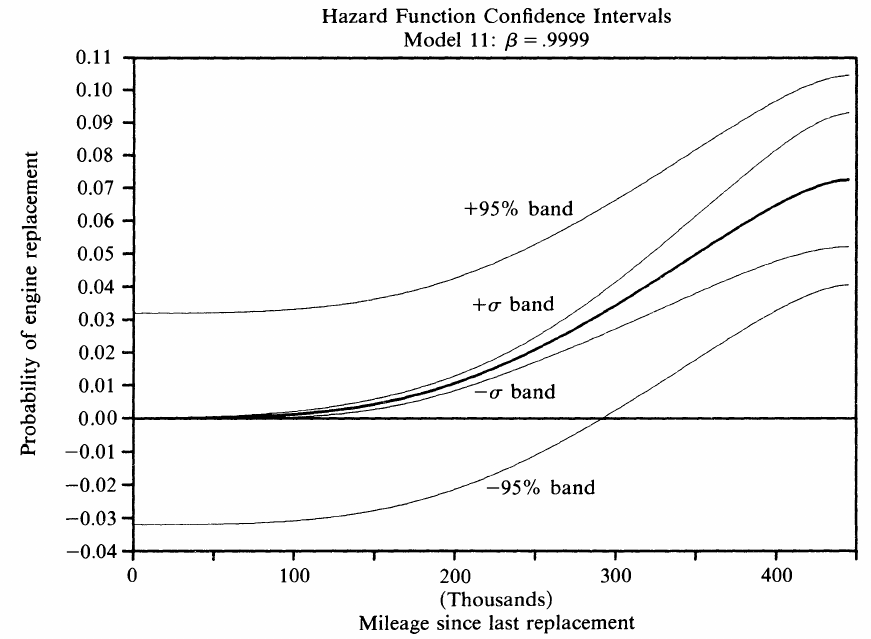
\includegraphics[width=0.9\textwidth]{hazard_function.png}
\end{frame}

\begin{frame}\frametitle{Mileage Distributions}
    \centering
    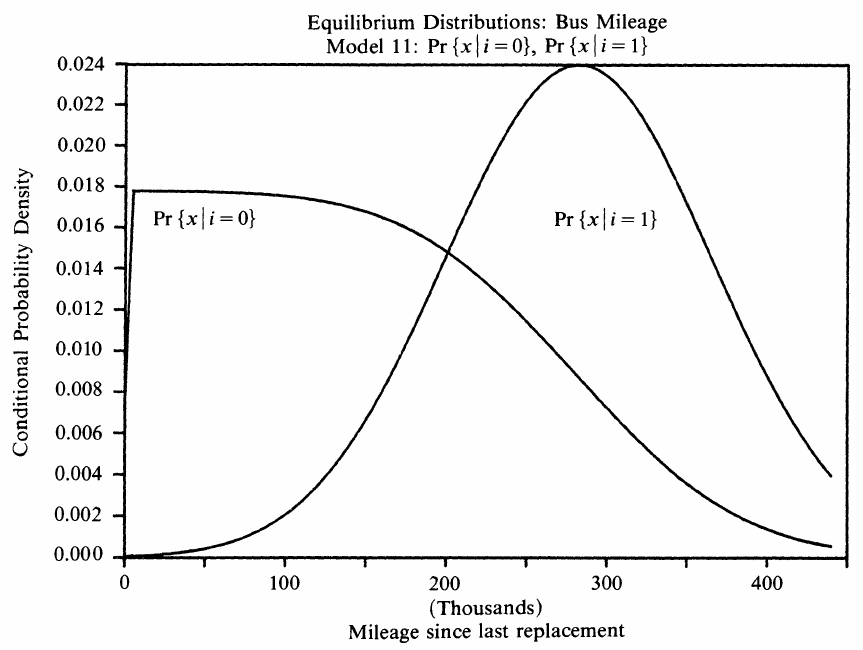
\includegraphics[width=0.9\textwidth]{mileage.png}
\end{frame}

\begin{frame}\frametitle{Engine Replacement Demand}
    \centering
    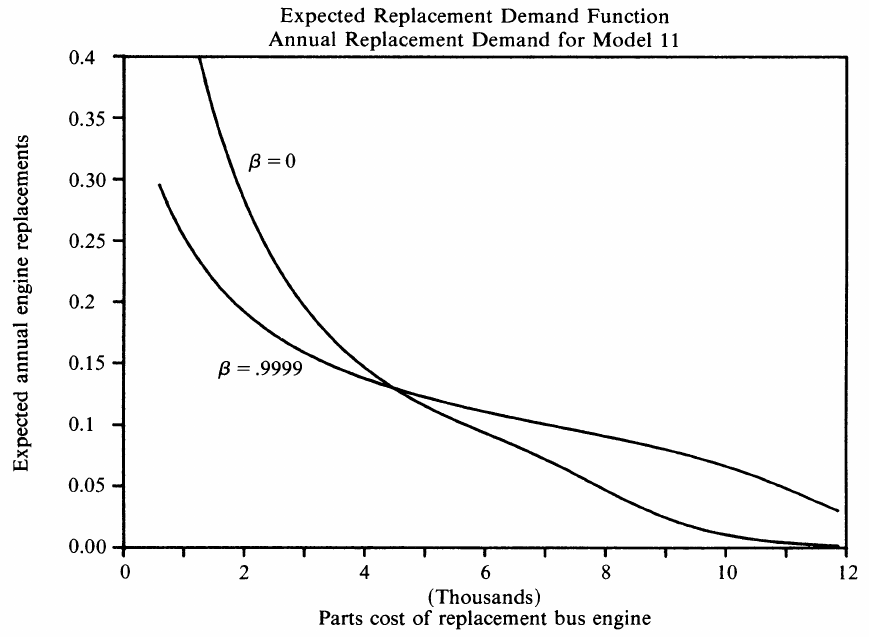
\includegraphics[width=0.9\textwidth]{demand.png}
\end{frame}

\begin{frame}\frametitle{Announcements}
    Reading for next time
    \begin{itemize}
        \item Train textbook, Chapter 13
         \item Nevo and Whinston (2010)
    \end{itemize}
    \vspace{3ex}
    Upcoming
    \begin{itemize}
        \item Final exam information next time
    \end{itemize}
\end{frame}

\end{document}